% Main document
\begin{document}
    % Add header
    \header{}

    % Use `answer` environment to add solutions
    % \begin{answer}[Question 1.1] for example starts an environment formatted
    % for Question 1.1
    \begin{answer}[Q1. Discuss and plot learning curves under $\epsilon$ values of $(0.1, 0.2, 0.3, 0.4)$ on MC, SARSA, and Q-Learning ]
        Your answer here.

        An equation with numbering:
        \begin{equation}
            \expdist{\sufstat}{\natparam}.
        \end{equation}

        An equation without numbering (notice the $*$):
        \begin{equation*}
            \expparam^{\T} \sufstat(x).
        \end{equation*}
    \end{answer}

    \begin{answer}[Q2. Discuss and plot loss curves under $\epsilon$ values of $(0.1, 0.2, 0.3, 0.4)$ on MC, SARSA, and Q-Learning]
        Your answer here.

        An equation with numbering:
        \begin{equation}
            \expdist{\sufstat}{\natparam}.
        \end{equation}

        An equation without numbering (notice the $*$):
        \begin{equation*}
            \expparam^{\T} \sufstat(x).
        \end{equation*}
    \end{answer}
    \begin{answer}[Q3. Discuss and plot $\text{...}$]
        Your answer here.

        \begin{figure}[H]
            \centering
            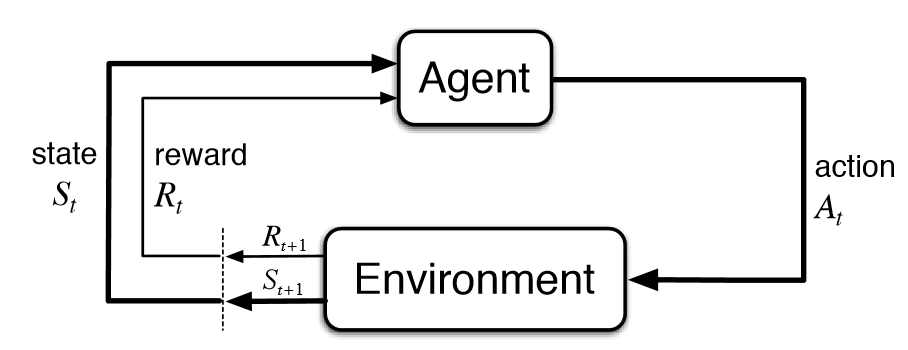
\includegraphics[width=0.5\textwidth]{images/RL_framework.png}
            \caption{Caption}
            \label{fig:enter-label}
        \end{figure}
        
        An equation with numbering:
        \begin{equation}
            \expdist{\sufstat}{\natparam}.
        \end{equation}

        An equation without numbering (notice the $*$):
        \begin{equation*}
            \expparam^{\T} \sufstat(x).
        \end{equation*}
    \end{answer}
\end{document}